\documentclass[11pt]{article}
\usepackage[top=0.70in, bottom=.80in, left=1in, right=1in]{geometry}
\renewcommand{\baselinestretch}{1.1}
\usepackage{graphicx}
\usepackage{natbib}
\usepackage{amsmath}
\usepackage{multicol}
\usepackage{tcolorbox}
\usepackage{caption}
\usepackage{todonotes}
\usepackage[font=sf]{caption}
\usepackage{hyperref}
\newcommand{\llabel}[1]{\hypertarget{lintarget:#1}{}\linelabel{lin:#1}}

\usepackage{lineno}
\renewcommand\linenumberfont{\normalfont\tiny\color{gray}}


\bibliographystyle{besjournals}

\begin{document}

% \title{Closing the gap between statistical and scientific workflows for improved forecasts in ecology} 
\title{Closing the gap between statistical and scientific workflows for improved inference in ecology} 
\date{\today}
\author{Victor Van der Meersch$^{1*}$, James Regetz$^{2}$, T. Jonathan Davies$^{1,3}$ \& EM Wolkovich$^{1}$}
\maketitle
\noindent $^{1}$ Forest and Conservation Sciences, University of British Columbia, Vancouver, BC V6T 1Z4, Canada\\
$^{2}$ National Center for Ecological Analysis and Synthesis, 1021 Anacapa St, Santa Barbara, CA 93101, United States\\
$^{3}$ Botany, University of British Columbia, Vancouver, BC V6T 1Z4, Canada \\
$^{*}$ \url{mailto:victor.vandermeersch@ubc.ca}\\

\noindent \emph{For:} Workflow for Applied Data Analysis theme issue for \emph{Phil Trans A} as an \emph{Opinion}

\begin{abstract}
% Concerns about increasing biodiversity loss and climate change have led to greater demands for useful ecological models and forecasts. Datasets relevant for developing these models and forecasts have also increased in size and complexity, including in their geographical, temporal and phylogenetic dimensions. New research often suggests that models accounting for these complexities can yield more accurate trends and predictions. We argue, however, that the usual workflows for model fitting in ecology make it difficult to evaluate and compare most current models for several reasons. First, the research community is split between two disconnected paradigms: either using data to fit simple, trend-like models with one or few parameters, or developing forecasting models that include complex, mechanistic, and/or black box submodels only indirectly informed by data. Second, in both cases, models tend to be developed not only in isolation of one another, but also without a coherent framework for linking scientific questions and understanding to statistical and modeling decisions, throughout the entire modeling process. We propose a unified, principled workflow for end-to-end empirical model development that bridges the gap between process-based and statistical approaches, integrates sound statistical and scientific practices, and especially relies on data simulation to inform decisions at multiple steps in the process. We argue that this approach, coupled with a shift toward universal training, more open model sharing, and alignment on common datasets, could transform for ecological modeling.
Concerns about increasing biodiversity loss and climate change have led to greater demands for useful ecological models. Datasets relevant for developing these models have also increased in size and complexity, including in their geographical, temporal and phylogenetic dimensions. New research often suggests that models accounting for these complexities can yield more accurate trends and predictions. We argue, however, that the usual workflows for model fitting in ecology make it difficult to evaluate and compare current models for several reasons. First, the research community is split between two disconnected paradigms: using data to fit simple, trend-like models with few parameters, or developing forecasting models that include complex, mechanistic submodels only indirectly informed by data. Second, in both cases, models tend to be developed not only in isolation of one another, but also without a coherent framework for linking scientific questions and understanding to statistical and modeling decisions, throughout the entire modeling process. We propose a principled workflow for end-to-end empirical model development that bridges the gap between process-based and statistical approaches, integrates sound statistical and scientific practices, and especially relies on data simulation to inform decisions at multiple steps in the process. We argue that this approach, coupled with a shift toward universal training, more open model sharing, and alignment on common datasets, could transform ecological modeling.


% jdavies15april: I feel this could be a critical step somehow - sharing simulations could allow cross-validation between models or perhaps cross-calibration ...
% These problems stem in part from continuing gaps between statistical workflows---where the data processing and model development are often addressed separately from the ecological question and aim---and scientific workflows, where all steps are integrated. Yet, as ecologists become increasingly computational the opportunity to close this gap has never been greater. We outline how increased data simulation at multiple steps in the scientific workflow could revolutionize our understanding of ecological systems, yielding new insights for both trend estimation and forecasting.
%Combining these changes with more open model and data sharing---and developing new efforts to race the same data---could be transformative for ecological forecasting. 
%A shift toward universal training in a more robust model building could bridge the gap between process-based and statistical approaches and be transformative for ecological modeling.
\end{abstract}

% {\noindent \bf Goal:} Increase awareness of how we can merge statistical and scientific workflows in ecology (especially forecasting) and what we would get out of it.
\linenumbers

\section{Introduction}

Anthropogenic drivers are reshaping natural systems \citep{Diaz2019}. Impacts are projected to increase in coming decades, as climate change accelerates biodiversity loss, altering ecosystem services and human well-being \citep{IPBES2019}.
Implementing sustainable policies to mitigate these impacts is thus a global priority, but designing the best policies requires estimating and understanding biodiversity and ecosystem trends to date, alongside the skill to forecast future dynamics. % These requirements in turn have created a growing need for more global ecological data, and the types of models that can robustly handle such data. 

Meeting these policy needs has led often to two separate paths: one focused on estimating trends from new global datasets, and another focused on forecasting from generally distinct datasets or mechanistic models based on less data. 
Newly available large-scale, long-term datasets have provided our first `global' estimates of biodiversity trends \citep[e.g.][]{loh2005living,Dornelas2018}, but these data---gathered opportunistically from multiple sources---are unbalanced and suffer from large geographic, temporal and taxonomic biases. Models to date have failed to fully address these challenges and, perhaps because of these limitations, are rarely if ever used for forecasting.
Instead, forecasting---under different plausible scenarios---has generally relied on entirely different datasets combined with either correlative or process-based models \citep{IPBES2019}, with process-based models often promoted as the most realistic approach \citep{Urban2016, Pilowsky2022} because they focus on mechanistic representations of ecosystem functioning. These approaches have failed to yield clear agreement on current species trends, leading to ongoing debates about the magnitude and even direction \citep{Dornelas2014, Leung2020, Buschke2021, Johnson2024}, and producing forecasts that diverge due to high model uncertainty at the ecological level \citep{Cheaib2012, Thuiller2019}.

\llabel{inferentialgoal}The inferential goals of these two modeling paradigms---explanation vs.\ prediction---seem disconnected at first glance, but remains in reality much more blurred. Trend estimation, often with simpler models, tend to focus on an explanatory purpose, but often lacks a clear link with theories that could provide causal interpretation. For forecasting, the use of more complex process-based models for a predictive purpose is often justified by the assumption that ``we must understand to predict", contributing to the confusion between explanation and prediction \citep{Shmueli2010}.

We argue that current debates, confusions and diverging forecasts are driven in large part by the incoherent and disconnected workflows used today in ecology \citep{Loreau2022, Talis2023, Johnson2024}. Research estimating biodiversity trends has become focused on methodological aspects; the current workflow fails to examine the gap between ideal and available data, and rarely tests for predictive accuracy that could scale up to allow forecasting. At the same time, process-based models developed for forecasting often evolve through the addition of new separate layers or components. These new parts are often disconnected from the original research aim, its data stream, and the previous scientific insights, because current approaches rarely examine the model as a functioning whole and thus ignore major problems (e.g., non-identifiability, discussed below).

Workflows that fully integrate all the steps required to build a model from an ecological question, with evaluation of limitations and potential problems before estimating its parameters and making projections, could reduce many of these problems. In particular, we argue that workflows that incorporate data simulation at multiple steps can quickly identify flaws in model structure and constraints in data, and allow us to understand when, where, and why different models diverge \citep{McElreath2018, betanworkflow,Gelman2020,Schad2020,grinsztajn2021,vandeschoot2021,Wolkovich2024}. Towards this aim, we outline the steps of a universal workflow that could harmonize both trend estimation and forecasting.

\section{Scientific method and workflows}

Quantitative science relies on a model-based framework to confront hypothesis with data \citep{Chamberlin:1965cd}. In an idealized scientific method, we would formulate a research question and hypotheses, design an experiment accordingly, build a model, collect data, and use this data to inform our model and differentiate between hypotheses. This method underlies much of the recent pre-registration movement, where hypotheses and methodology are defined prior to data collection \citep{Nosek2018}.
But this idealized method often does not apply to the reality of ecological research. Many important questions cannot be addressed through controlled experiments and replications. In such cases, we must rely on existing, heterogeneous datasets alongside uncertain and incomplete theory to provide a large-scale and long-term perspective \citep{Hilborn1997}. Indeed, most macroecological insights have emerged from exploring patterns in these datasets (exploratory data analysis).

\begin{figure}[h]
	\centering
	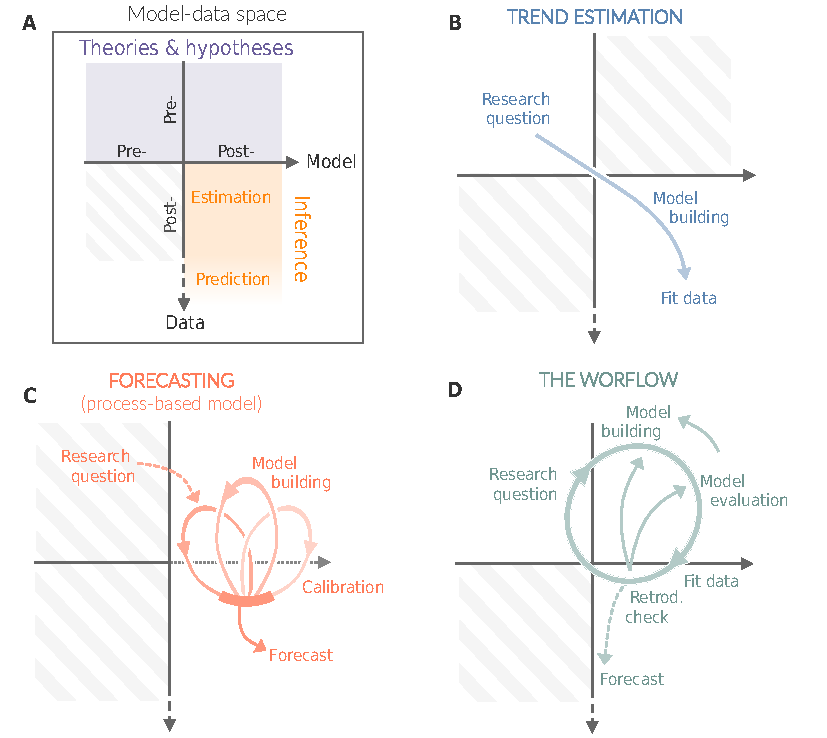
\includegraphics{../figures/figure_modeldataspaces_revised}
	\caption{Different trajectories through model-data space during model development, from pre-model/pre-data to post-model/post-data quadrants.
	Panel A serves as a legend, showing where model development should begin (carefully thinking about the hypotheses we want to test) and when inference should be made, for either explanatory purpose (estimation) or forecasting (prediction).
	Panel B illustrates that in current trend estimation approaches, most time is spent in the post-model/post-data quadrant, where models are directly fitted to empirical data---often with no prior evaluation of the model.
	Panel C illustrates the typical process-based model development. A lot of time is spent building and calibrating (fitting) separate submodels, without clear distinction between model building and model calibration and without evaluating the full model structure a priori. Additionally, the specific hypotheses the model is designed to test are rarely clearly stated.
	Panel D illustrates the workflow highlighted in this paper (see main text and Figure 2 for details). Ideally, it begins in the pre-model/pre-data quadrant, where the research question is defined. The next step moves to the post-model/pre-data quadrant, where a model is built---independently of the data. This is where we should spend a good deal of time evaluating model behavior using simulated data. Once we are satisfied with our model, we can move to the post-model/post-data quadrant, where the model is fitted to real data. Then, we perform retrodictive checks to compare model predictions to observations, which likely give us some feedback to refine our model.}
	\label{fig:modeldata}
\end{figure}

This reality should drive researchers to use more robust and coherent methods. But the current workflows combined with the challenges ecologists are facing---both in terms of data complexity and societal needs---instead may lead to persistent problems.
Trend estimation has focused mostly on fitting a model to empirical data (\llabel{quad1}i.e. post-model/post-data, figure \ref{fig:modeldata}b)---without the checks (\llabel{quad2}post-model/pre-data) and likely feedbacks that often highlight uncertainty and related limitations in the model and/or data (figure \ref{fig:modeldata}b). For forecasting, researchers have focused on making predictions with increasingly complex mechanistic models (figure \ref{fig:modeldata}c), frequently obscuring the steps underlying model building and parameterization (\llabel{quad3}and without a clear distinction between pre- and post-data). Researchers often calibrate the different parts of these models separately, and fix some parameter values based on experiments and expert knowledge, to avoid problems when trying to fit the model as a whole.
Addressing these problems while accounting for the realities of working with ecological data requires a more comprehensive workflow.

We argue a workflow that moves \llabel{quad4}along the data-model space in a coherent sequence of steps (figure \ref{fig:modeldata}d) could reduce many of these problems and thus improve ecological science.
The first step of this workflow is to define an explicit research question and formulate hypotheses (step 1, figure \ref{fig:workflow}). This involves making clear assumptions about the most influential drivers, within the specific context of our study. This should guide the construction of a narrative model of how we believe the system works, focusing on the mechanisms that could generate the data we observe, including the observational error (\llabel{quad5}pre-model/pre-data, figure \ref{fig:modeldata}d).  
\llabel{causalinf}This step of carefully formulating hypotheses has gained increasing attention in the ecological literature \citep{Grace2020}. From this narrative, we can then develop a mathematical model---an ensemble of equations that encapsulates our knowledge and is designed to answer our research question (step 2, figure \ref{fig:workflow}). The general idea is to start with a relatively simple model that we could refine later (see example workflow we provide). At this stage, prioritizing biologically meaningful parameters is crucial, as it allows us to have a sense of plausible parameter values. This means choosing a model formulation where each parameter corresponds to an interpretable behavior (which sometimes requires considering alternative parameterizations). 

With a model in place, the next step focuses on testing and understanding it via data simulation (step 3, figure \ref{fig:workflow}). `Fake' or `test' data are generated directly from the model by fixing parameters \llabel{firstsim}to some reasonable values (which is straightforward if the parameters are interpretable) and from fake predictor data. 
We then fit our model to this simulated dataset and evaluate its ability to recover the prescribed values (\llabel{quad6}post-model/pre-data, figure \ref{fig:modeldata}d). At this stage, the focus is on understanding the model, so we may need to spend time thinking about whether each parameter is realistic or not. This is also a step for making sure the model is working as expected (see example worklow). \llabel{repeatsim}Ideally, this data simulation step should be repeated several times with different parameter values, sampled within a reasonable range. \llabel{priorPC}In a Bayesian framework, simulated parameters can be sampled from the prior distribution (allowing us to check the implications of our priors, \citealp{Gelman2020}).

Once we are confident about our model structure, we can introduce real data as part of an initial model fitting step (step 4, figure \ref{fig:workflow}). This way, we obtain parameter estimates constrained by observations (\llabel{quad7}post-model/post-data, figure \ref{fig:modeldata}d). 
These parameter estimates lead to the second data simulation step, this time using our fitted model parameters to generate predictions (step 5, figure \ref{fig:workflow}). This---which we call a retrodictive check (\citealp{betanworkflow}, also called a \llabel{PPC}posterior predictive check in a Bayesian workflow,  \citealp{Gelman2020})---allows model output to be compared to observations. \llabel{howtoPPC}There is no general way to do this: the goal is to tailor checks that assess key features of the data in regards to our research question \citep{Gelman2020}.
It's only once all steps have been completed that we can interpret parameter values with respect to our research question.
The workflow encourages a focus on the full model, where any parameter (such as a trend estimate) must be carefully interpreted alongside others, as all are fundamental components that shape both inference and forecasting. 

Within such a workflow, forecasting emerges as a natural outcome: rather than being a final goal, it only involves jointly modeling new circumstances along with the original data. The adoption of the workflow in macroecological studies---where model building is often informed by patterns in the data---would also make the exploratory analysis more transparent (as an explicit preliminary step for entering the workflow) and would compel researchers to more clearly develop a research question before extensive model fitting. 

A key feature of this workflow is the central role of data simulation, which introduces two feedback loops---\llabel{broadcontext}and should be applied not only in a Bayesian framework but across broader modeling approaches.
The first feedback arises when we evaluate the model on simulated data.
The failure of the model to recover known parameter values and handle the complexity of the simulated data should prompt reconsidering the model, or even reformulating the research question.
Further, this step might reveal that some parameters are highly non-identifiable (meaning the parameter(s) cannot be uniquely estimated),
flagging the need to change the model structure---before incorporating empirical observations. 
The second feedback loop comes from the retrodictive check. 
Discrepancies here may indicate a missing key driver, and suggest the current model is too simplistic. We can refine the model to integrate the missing process(es) (if we can identify them) and return to the start of the workflow. Insights from the retrodictive check can also lead us to introduce additional complexity when simulating fake data, such as phylogenetic structure or observational biases (e.g. unbalanced data). For example, if a researcher realizes their empirical data is geographically biased, this bias should be built into the model and thus into this data simulation step. This iterative evaluation of the model moves beyond a simple reliance on goodness-of-fit metrics. At each iteration, we are able to evaluate the model behavior, both with simulated and real data, taking into account our expert knowledge of the ecological processes. 

\begin{figure}[h]
	\centering
	\vspace*{-0.1cm}
    \hspace*{-1.5cm}
	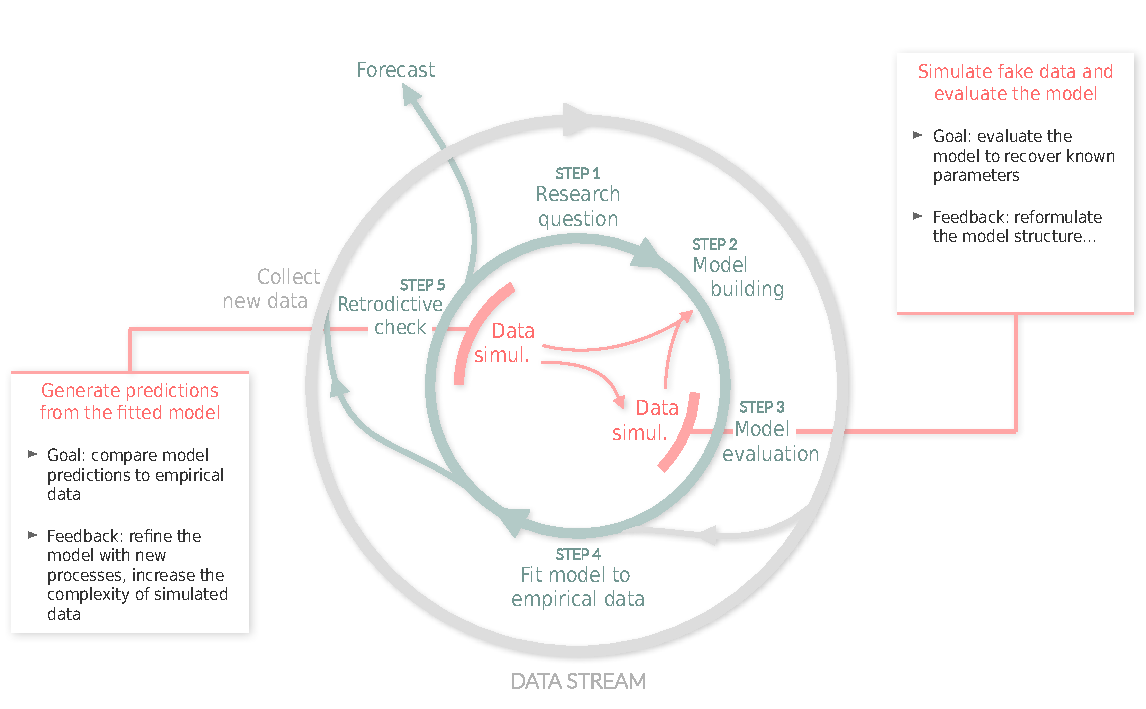
\includegraphics{../figures/figure_worflow_wsteps}
	\caption{The workflow we propose here \citep[which builds from recent advances in workflows,][]{betanworkflow,Gelman2020,Schad2020,grinsztajn2021,vandeschoot2021,Wolkovich2024} focuses on iterative feedbacks between the research question, model and data. Most research should start at Step 1, with the research question, followed by extensive model building and evaluation using simulated data (Steps 2 and 3) before proceeding to fitting the model on empirical data and examining it through retrodictive checks (Steps 4 and 5). Within this workflow, forecasting is a natural output of the process and not a separate process or one available for only certain modeling approaches.  The integration of observations (the data stream) occurs at Step 4---only after the model has been thoroughly evaluated---and can also highlight opportunities to collect new data and enrich the data stream.}
	\vspace*{-0.5cm}
	\label{fig:workflow}
\end{figure}

\section{The workflow in practice}

Across the different fields of ecology---for both parameter estimation and forecasting---a systematic application of a coherent workflow could highlight the best opportunities to accurately \llabel{quant1}quantify uncertainties and yield new scientific insights. This will help refocus the debate on designing new hypotheses, formulating new questions---and guiding efforts to collect new data. Here, we illustrate how such a workflow could lead to significant improvements in two case studies: (i) estimating global biodiversity trends and (ii) forecasting future species and ecosystem dynamics using process-based models.

\subsection{Trends}

Ecologists today have amassed data on populations and species across the globe; they have also engaged in an increasing number of debates on regional and global trends over time, with arguments over the magnitude and even direction of population and biodiversity metrics \citep{Dornelas2014,Leung2020,terry2022no,muller2024weather}. While shifting estimates are part of the process of science---refining our approaches and thus estimates over time---we believe these debates would be fewer and they would be more rapidly resolved through use of an improved workflow. % Further, an improved workflow could give more rapid and coherent estimates, which could make it easier for  policy-makers to develop and advance initiatives aimed at slowing declines.

An improved workflow that required data simulation and retrodictive checks would lead to larger model advances and a greater recognition of uncertainty---thus highlighting likely consistency in estimates across models---that could better aid policy.  Using the workflow would make it more obvious that what now appear as major discrepancies are shifts in point estimates that are generally all in the same uncertainty space \citep{Johnson2024}---and it would challenge modelers to show major predictive advances, which is not currently part of the process. Explanatory power in most models of observational data is usually very low \citep{low2014rising,moller2002much} and thus tests of models' predictions rarely expected. But the workflow highlights that predictions from the model---what we call retrodictive checks---are part of the process of science, and critical to testing for what may be missing in a model. We expect retrodictive checks on most published trend analyses would highlight major missing components in these models, and drive changes both in the models themselves and in the simulated data to check the models. This step builds somewhat on the skills needed for null models \citep{Gotelli:2012oz}, but with a shift in focus towards the specific bespoke model at hand. Ecologists have started to use simulated data more to understand potential limitations of their models and data combined, but this is still extremely rare, and efforts to date often treat simulations as separate from the statistical model \citep{Buschke2021,dove2023quantifying}, short-circuiting their full utility if used in an iterative workflow.

Applying the workflow to current trend estimates could importantly highlight the best way to improve data collection for more reliable estimates. Returning to the example of a global estimate of trends in vertebrate populations of species over time (see Box) and applying our proposed workflow would mean more efforts to define the goal and question---is it a simple global estimate?
Or a need to also find which species are declining most, including those that may have poor or no data? From there a generative model using simulated data for testing could incorporate many aspects of the populations, and data, that are often only included in `null' or 'synthetic data generation' currently \citep{Buschke2021,mcrae2025utility} but could be built into the models fit to the empirical data. Eventually fitting the empirical data and performing retrodictive checks would likely highlight major missing components of the generative model and, ultimately, this would help inform our global estimates of mean trends (see workflow example). For example, certain populations are recovering for very specific reasons (e.g., elephants in regions where the ivory trade drove declines in the past) that perhaps should be modeled. From this model, what data are most critically needed to address the updated aims would become clearer and could drive new data collection \citep{toszogyova2024mathematical}. 

\subsection{Forecasting from process-based models}

Ecological forecasting is a broad field with a diverse range of methods. Our second case-study focuses on process-based modeling, which is often considered the gold standard for forecasting in ecology \citep{Urban2016, Pilowsky2022} and beyond. Newer models, however, generally incorporate greater complexity (and an ever-growing number of parameters), which can make it difficult to increase scientific understanding \citep{Franklin2020}, and suggest or model potential policies. 

Increasing model complexity can be beneficial, especially when it helps better \llabel{quant2}quantify the uncertainty; however, this is not always the outcome. In process-based modeling for climate forecasts, the uncertainty range on the effect of increasing CO$_{2}$ concentration on temperature have remained largely unchanged \citep{Zelinka2020}. This has driven calls for more rigorous and transparent calibration processes \citep{balaji2022general}. Similar concerns arise in ecology, where strong disagreements exist about the effect of climate change on future species distributions \citep{Cheaib2012} and ecosystem dynamics \citep{Lovenduski2017}.
These uncertainties have large implications beyond ecology, as they influence simulations of biosphere-atmosphere interactions and, ultimately, future climate projections \citep{Bonan2018, simpson2025confronting}.
Some researchers now advocate for simplifying models, to avoid over-parametrization when the data provide little information to constrain some parameters \citep{Wang2017, Harrison2021}. 
If a model becomes too complex, it may become a black box,
and understanding the sources of uncertainty and how they propagate through the model may become nearly impossible (see Box).
Each additional process and parameter can increase overall uncertainty to the point where model projections lose their usefulness for decision makers \citep{Saltelli2020}. 

Process-based models used to project species or ecosystem distributions highlight some of these problems. Most of the focus is on the model projections---often represented as maps without uncertainties. Model evaluation generally focuses on how well these projections match observed distributions, sometimes under different climatic conditions to challenge the models \citep{VanderMeersch2025a}---most of the time evaluating only one of the many different output variables of the model.
The complexity of these models can make it difficult to assess how well the potential parameter space was searched, and whether there was any potential non-identifiability---such work is generally done as a separate effort, exposing potential model problems later on \citep{VanderMeersch2025b}, and not required as a preliminary step. 

Applying the workflow to process-based models would help open the black box.
Each successive step of model development in the workflow may highlight current problems and a path to solutions. Incorporating data simulation would introduce a crucial step between model building and data fitting (also called calibration), ensuring a clear delineation between the two, and help expose potential parameter identifiability issues in the model design. 
Uncovering identifiability issues would likely force researchers to begin with a simpler version of the model, which they could build on iteratively, testing for support---or lack thereof---when adding model complexity. The workflow may also highlight model problems by requiring more explicit model calibration (i.e. data fitting), which is currently hidden within opaque `model building', making it easy to hide non-identifiability in the model. Through the workflow non-identifiable parts of models could be addressed by reformulating the mathematical structure of certain processes, or finding ways to apply additional constraints (e.g., narrower ranges for certain parameters or developing new hypotheses that target the appropriate level of complexity). The resulting process-based models would likely be simpler and thus more tractable for quantifying parameter uncertainty and propagating it through projections. 

% Box
% \setlength{\columnseprule}{0.1pt}
\begin{tcolorbox}[
sharp corners=all,
colback=white,
colframe=black,
size=tight,
boxrule=0.1mm,
grow to left by=+1cm, grow to right by=+1cm,
enlarge top by=-1.2cm,
left=3mm,right=3mm, top = 2mm, bottom = 2mm,
fontupper=\footnotesize
]
{\begin{multicols}{2}

\centerline{\bf Trend estimation}
\vspace*{2mm}
\begin{minipage}[t]{\linewidth}
    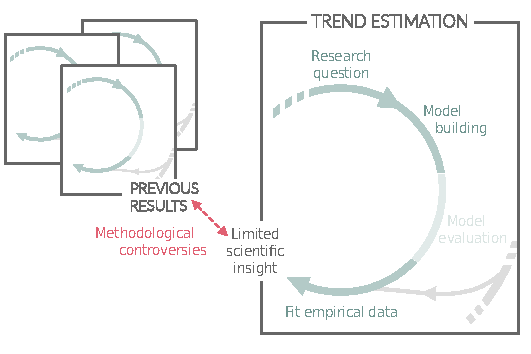
\includegraphics[width=\linewidth]{../figures/trendestimation_details}

    % \vspace{-0.5cm}\captionsetup{font=footnotesize}\captionof{figure}{Caption}\label{fig:trends}
    \vspace*{1mm}
\end{minipage}

% Trends - outline current problem
In the current workflow for estimating trends over time, a new model with a new estimate often leads to a paper (see figure A above) because ecologists spend less time interrogating their models with simulated data, or their model performance fit to empirical data. 
The Living Planet Index (LPI, \url{www.livingplanetindex.org}), which aims to include long-term data on vertebrate populations of species across the globe, is emblematic of these conflicting results. % \todo[]{could highlight how influential the LPI has become (recent reports suggest a 73\% ave. pop decline since 1970. This would be massive!}
With updated data released semi-annually alongside new datasets and new estimates of decline, a growing number of high-profile papers have challenged how strong the evidence is for population decline \citep{Dornelas2014,gonzalez2016estimating,wagner2021insect,muller2024weather}, with each paper taking a slightly different analytical approach. For examples using LPI data, \citet{Leung2020} published a mixture model that suggested most populations were not significantly declining, followed by other alternative modeling approaches \citep{Buschke2021,puurtinen2022living} including a recent one suggesting a basic analysis of the dataset should always include three sources of autocorrelation, finding trends that encompassed many previous results \citep{Johnson2024}. 


\vfill

\columnbreak

\centerline{\bf Mechanistic forecasting}
\vspace*{2mm}
\begin{minipage}[t]{\linewidth}
    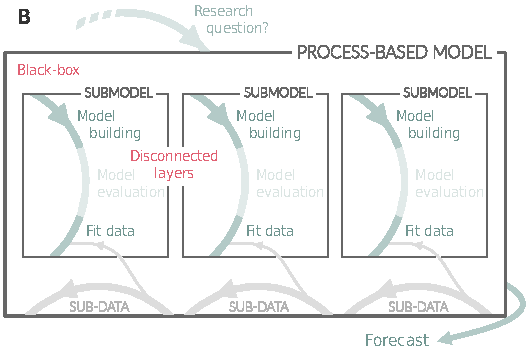
\includegraphics[width=\linewidth]{../figures/forecasting_details}

    % \vspace{-0.5cm}\captionsetup{font=footnotesize}\captionof{figure}{Caption}\label{fig:trends}
    \vspace*{1mm}
\end{minipage}

\noindent % Process-based models are built on explicit mathematical equations to describe (supposedly causal) relationships between environmental drivers and ecological responses. 
% They also often incorporate empirical relationships, particularly when knowledge is incomplete or when some processes are intentionally omitted. Processes are often represented at different nested spatiotemporal scales, depending on the underlying assumptions. 
Model development is the central step of the process-based workflow, typically requiring several years, yet it often remains opaque for anyone who has not worked the model itself. The step of designing the model---translating knowledge and hypotheses into mathematical equations and parameters---is often blurred with the step of model calibration (or tuning), where parameter values are inferred. Models are often treated as an accumulation of multiple submodels, each governing one or several ecological processes (see figure B above). Rather than being fitted as a whole, submodels are calibrated separately against specific subsets of data, and some parameters are simply prescribed (i.e., fixed to a value found in the literature) or tuned to reproduce certain observations or theory. The way models are currently calibrated is likely not a coincidence, but rather a workaround to avoid confronting the full complexity of the model. Calibrating submodels separately allows to avoid the fact that, if the model were fitted as a whole, many parameters would compensate for one another---revealing structural degeneracies and making the model far more difficult to use.

\vfill

\end{multicols}}

\centerline{\bf A common workflow to bridge trend estimation and forecasting} % jdavies15april: would it be possible to label this panel with components of the LPI to provide a clearer illustration of how the framework is implemented? % [FLAG: not sure I understood]
\vspace*{-3mm}
{\begin{multicols}{2}
\begin{minipage}[t]{\linewidth}
	\vfill
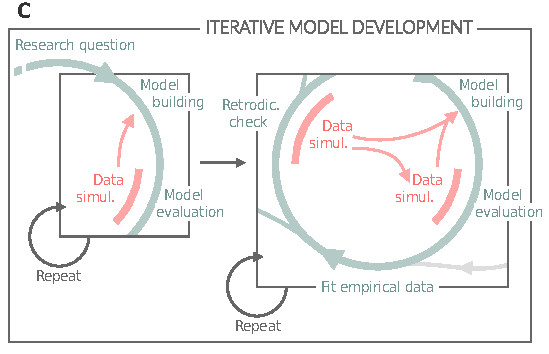
\includegraphics[width=\linewidth]{../figures/iterativeworkflow_details}
\vfill
% \vspace{-0.5cm}\captionsetup{font=footnotesize}\captionof{figure}{Caption}\label{fig:trends}
\vspace*{3mm}
\end{minipage}

\columnbreak
\vspace*{1mm}
A universal workflow offers an opportunity to bridge statistical and process-based frameworks, integrating mechanistic knowledge and leveraging robust statistical approaches \citep[e.g.][]{rounce2020quantifying}. Process-based models would no longer be perceived as deterministic black boxes by other researchers but rather as robust statistical frameworks encapsulating both data structure and mechanistic knowledge---and where the full model is fitted jointly. It would be an opportunity to spread the incorporation of mechanistic assumptions beyond the process-based modeling community, potentially improving trend estimates. For both trend estimation and forecasting, the workflow would refocus attention on the research question, highlighting the ecological hypotheses that justify the use and design of the model.

\end{multicols}}

\end{tcolorbox}

\clearpage
\section{Barriers and opportunities}

We believe our workflow could help advance ecological science and its applications, but widespread use of it requires overcoming major hurdles that pervade science.  
The first is pressure to publish quickly, which can be at odds with the reality that good model fitting is inherently iterative and takes time. The second is reluctance to embrace adoption of open science practices that ensure modeling efforts are fully transparent and reproducible. 
We believe adopting a workflow such as the one we propose may change this reluctance, and aligns with ongoing efforts to place increasing value on research that is carefully developed, openly collaborative (including both data and code), and transparent about areas of uncertainty.

\subsection{Adopting the workflow}

Advancing ecology to where most researchers use models built more flexibly from ecological theory and insights applied to their ecological systems will not happen rapidly without a major shift in training. Much of ecology still divides the world into training for those who gather data and learn a limited set of pre-built models versus those who develop more complex models. In ecological training today, researchers who conduct field and lab studies often learn a limited set of particular statistical tests matched to particular experiment designs and simple information on their variable types (e.g., categorical $x$ and $y$ leads to using a chi-squared test).

When ecologists trained in a limited set of tests require more complex models, they are expected to collaborate with others trained more in model development (though often for highly specific applications, such as wildlife population estimates, where generative models are often predefined). These two groups further differ from process-based modelers, who often train in physical and ecophysiological processes and how to abstract them into mainly deterministic models.
Neither group has fully integrated data simulation into their statistical or scientific workflows. Simulation is generally reserved as a form of training needed mainly by those specializing in theoretical ecology, who often solve analytical equations but rarely link to empirical data. While specialization is valuable, we argue the fundamental % training
separation in ecology has overly-siloed these groups and prevented more rapid progress.

We suggest unified training in our proposed workflow, or a similar one \citep{betanworkflow,Gelman2020, grinsztajn2021,vandeschoot2021}, would focus on learning to generate questions and then models, and then how to simulate data from them. Through this and the use retrodictive checks, most ecologists would be better equipped to think through what parameters are most critical to their question and/or aim (e.g., management), and also gain a much stronger connection to the level of uncertainty in many of ecological estimates. Empiricists would be more likely to recognize critical gaps in current models fit by those specializing in ecological modeling and help advance those models. Process-based modelers may start a new generation of simpler models that are more tractable to theoretical ecologists, who may see new bridges from their work to empirical data and forecasting.

\subsection{A tractable alternative to machine learning}

With rapid advances in machine learning, improving current methods to gain greater scientific insights to drive better forecasting seems increasingly important. \llabel{MLvsPBM}Machine learning will likely surpass process-based models for forecasting accuracy if the latter lack a robust estimation of their parameters and fall in a complexity trap, at the cost of their interpretability. Similarly, estimates of trends from empirical data using models without clear mechanistic drivers may soon offer fewer advantages over machine learning. 

Beyond improving model building and evaluation, our proposed workflow also has the potential to shift how process-based models are perceived, particularly by those unfamiliar with them.
Process-based models could once again be a way to answer a research question---whereas today, model simulations have increasingly become a subject of study on their own.
Ideally, applying the workflow would help to move away from the traditional process-based model paradigm, where parameters are typically assigned fixed values without properly accounting for their uncertainty. Instead, it would guide a step-by-step model fitting, parameter estimation, and uncertainty quantification---preventing modelers from making biased inferences and unfounded assumptions beyond what the data can support. It would thus define a clear and limited context in which the model should apply, and limit discussion of adding increasing complexity. 

\emph{Conclusions:} 
Today model development in ecology is rarely transparent, which limits how easily the research community can understand models, and thus identify potential issues. Instead of broad inclusive conversations about how to improve models to advance our ecological understanding, a significant portion of scientific debate has become mired in methodological considerations. However, we believe our workflow provides a tractable step to fixing this. By focusing on model development more tightly tied to ecological expertise, we argue this workflow should broaden the community that contributes to model development. It may also help resolve apparent conflicts by identifying where divergences in model predictions emerge, whether from differences in assumptions, model structures, or other aspects of the modeling process.
As ecologists are increasingly expanding their computational toolkits, many field, and lab, and other forms of `empirical' ecologists have the basic tools to follow this workflow to build models that better represent their ecological domains of interest, and---most importantly---to interrogate those models.

% This shift would present a significant challenge---as it would likely reveal many issues related to non-identifiability in models and data limitations before achieving robust inference. But ultimately, it would prevent modelers from making biased inferences and unfounded assumptions beyond what the data can support.

\clearpage
\bibliography{../forecastflows.bib}

\end{document}
